\scanpage{14}
$G_Q$ le graphe associé à un carré combinatoire $Q$,
\figure{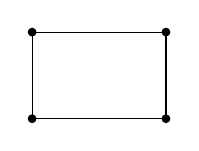
\begin{tikzpicture}\draw (0,0)--(1.7,0)--(1.7,1.1)--(0,1.1)--cycle;\fill (0,0) circle(1.6pt);\fill (1.7,0) circle(1.6pt);\fill (0,1.1) circle(1.6pt);\fill (1.7,1.1) circle(1.6pt);\end{tikzpicture}}
Soit $\operatorname{diag}Q$ l'ens des deux diagonales de $Q$; $\unsure{\mathcal A|A}(Q)$ l'ens des quatre côtés, s'identifie à
\[
\unsure{\mathcal A|A}(Q)=\prod_{\Delta\in\operatorname{diag}Q}\Delta
\]
\margin{\deleted{ens sur lequel}\inserted{torseur sous} $\{\pm1\}^{\operatorname{diag}Q}$, \deleted{qui} \unsure{donc|dont} $\{\pm1\}\subset\{\pm1\}^{\operatorname{diag}Q}$ y opère}
\deleted{\unsure{qui se}} qui se groupent \deleted{\unsure{en}} par paires de côtés opposés, en codiagonales. Alors
\[
\operatorname{codiag}(Q)\simeq\bigwedge_{\Delta\in\operatorname{diag}Q}\Delta
\]
On a ici, en termes du graphe $G_Q$
\[
\begin{aligned}
S&\simeq\operatorname{diag}Q&&\text{soit }\Delta_s\text{ la diagonale associée à }s\in S\\
I&=A^{\mathrm{lib}}=\unsure{\mathbf I|I}(Q)&&\text{ens des }\deleted{\text{côtés orientés}}\inserted{\text{sommets}}\text{ de }Q\\
\widehat{\vec A}&\simeq\mathbf I\amalg\widetilde S&&\substack{\text{en associant à }s\in S\text{ l'arête}\\\text{orientée liée }\widetilde s\text{ d'origine }s}\\
\widehat{\vec A}_s&=\Delta_s\amalg\{\widetilde s\}&&\text{donc }\varepsilon_s=\omega(\widehat{\vec A}_s)\simeq\Delta_s\\
\varepsilon_{(G)}&\simeq\prod_{s\in S}\Delta_s\simeq A(Q)&&\text{en tant que torseurs}\\
\gamma_G&=\prod_{s\in S}\{\pm1\}=\{\pm1\}^{S}.&&
\end{aligned}
\]
On trouve $S_0\mathcal T_G$ à l'aide de l'extension $\mathcal E_{G^b}$
\[
0\longrightarrow\mathbb Z^S\xrightarrow{2}\mathbb Z^S\longrightarrow\overbrace{\{\pm1\}^S}^{\gamma(G)}\longrightarrow0
\]
et du \inserted{$\gamma(G)$-torseur} $\varepsilon(G)$, en prenant $\mathcal E_{G^b}(\varepsilon(G))$, ce qui donne un $\mathbb Z^S$-\unsure{groupoïde}\inserted{sur $\gamma(G)$}, et en faisant l'extension du groupe \unsure{central} $\mathbb Z^S$ à $\mathbb Z^{\widehat{\vec A}}$, par
\mspage{13}
